% =====================================================================
% figures.tex —— ACL_PAPER_ZH 的全部图环境(LaTeX 侧直接 \input 或复制)
% 前置要求: \usepackage{graphicx} \usepackage{booktabs} \usepackage{amsmath}
% 宽度: 单栏图 \columnwidth ≈ 3.3in; 双栏图 \textwidth ≈ 6.8in(figure*)
% =====================================================================

% ---------- Figure 1 主图(双栏) ----------
\begin{figure*}[t]
  \centering
  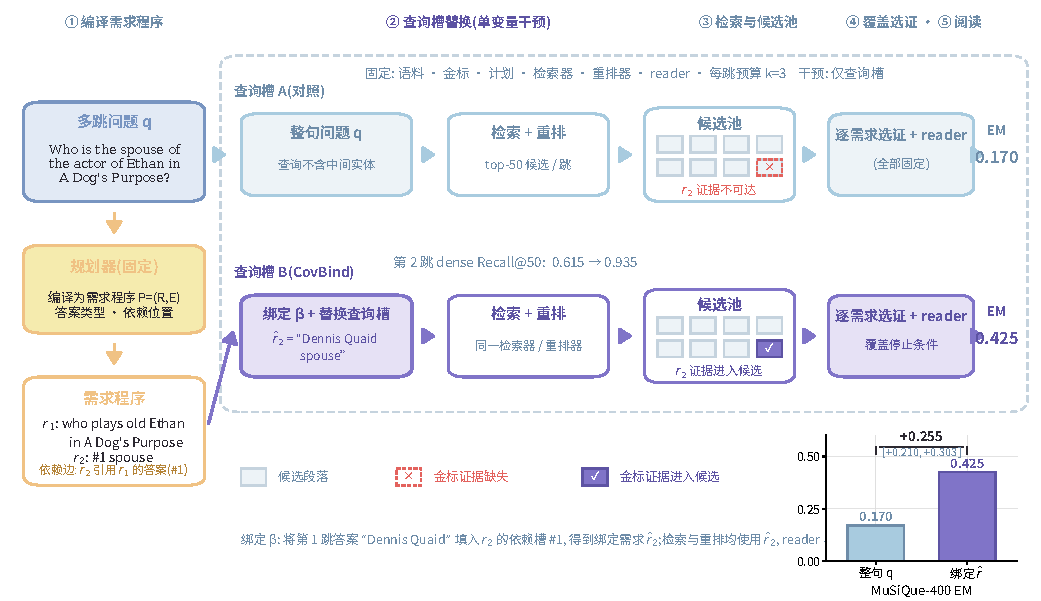
\includegraphics[width=\textwidth]{figures/fig1_method_overview.pdf}
  \caption{CovBind 总览与查询槽单变量反事实。左侧将多跳问题编译为带依赖边的需求程序;
  中部虚线框内为干预实验:固定语料、金标、计划、检索器、重排器、reader 与每跳预算,
  仅替换检索与重排使用的查询槽——上分支使用整句问题(对照),下分支使用前序答案绑定后的
  需求 $\hat{r}_2$(CovBind)。绑定使第 2 跳 gold 证据重新进入候选池(dense Recall@50:
  $0.615\!\to\!0.935$),端到端 EM 从 $0.170$ 提升至 $0.425$(MuSiQue-400,配对 bootstrap
  95\% CI $[+0.210,+0.303]$)。右下角为对应配对结果。}
  \label{fig:method}
\end{figure*}

% ---------- Figure 2 查询槽反事实(单栏) ----------
\begin{figure}[t]
  \centering
  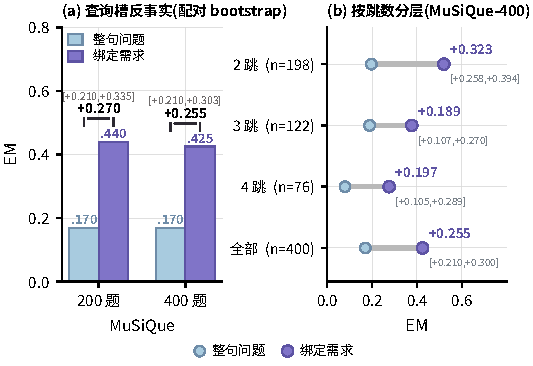
\includegraphics[width=\columnwidth]{figures/fig2_queryslot_counterfactual.pdf}
  \caption{查询槽反事实。(a) MuSiQue 200/400 题上,仅将查询槽从整句问题替换为绑定需求,
  EM 分别提升 $+0.270$ 与 $+0.255$(95\% CI);(b) 按跳数分层后收益依然稳定:
  2/3/4 跳分别 $+0.323$、$+0.189$、$+0.197$。浅蓝点为整句问题,紫色点为绑定需求。}
  \label{fig:queryslot}
\end{figure}

% ---------- Figure 3 逐跳可达性(单栏) ----------
\begin{figure}[t]
  \centering
  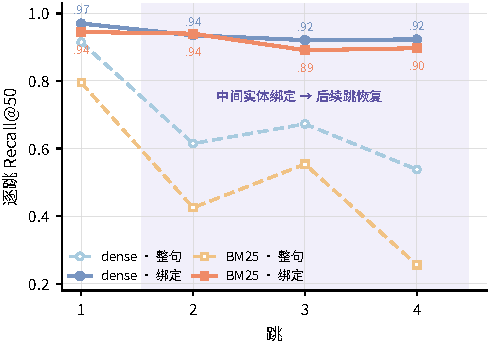
\includegraphics[width=\columnwidth]{figures/fig3_hop_reachability.pdf}
  \caption{绑定恢复后续跳的候选可达性(逐跳 Recall@50)。第 1 跳提升来自需求聚焦;
  第 2--4 跳的大幅恢复来自中间实体绑定:dense 从 $0.538$--$0.673$ 恢复至
  $0.921$--$0.935$,BM25 从 $0.256$--$0.554$ 恢复至 $0.891$--$0.940$。}
  \label{fig:reach}
\end{figure}

% ---------- Figure 4 可达性×选择效率(单栏) ----------
\begin{figure}[t]
  \centering
  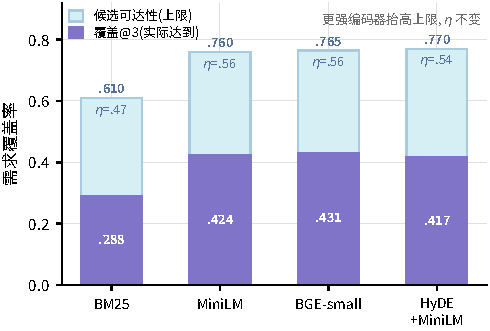
\includegraphics[width=\columnwidth]{figures/fig4_reach_efficiency.pdf}
  \caption{覆盖损失分解:候选可达性(浅色柱,上限)与覆盖@3(深色柱,实际达到)。
  BM25、MiniLM、BGE-small 与 HyDE+MiniLM 的候选可达性为 $0.610$--$0.770$,
  但逐点选择效率 $\eta$ 长期停留在 $0.47$--$0.56$:更强编码器抬高上限,
  而选择效率基本不变。}
  \label{fig:decomp}
\end{figure}

% ---------- Figure 5 覆盖瓶颈(双栏) ----------
\begin{figure*}[t]
  \centering
  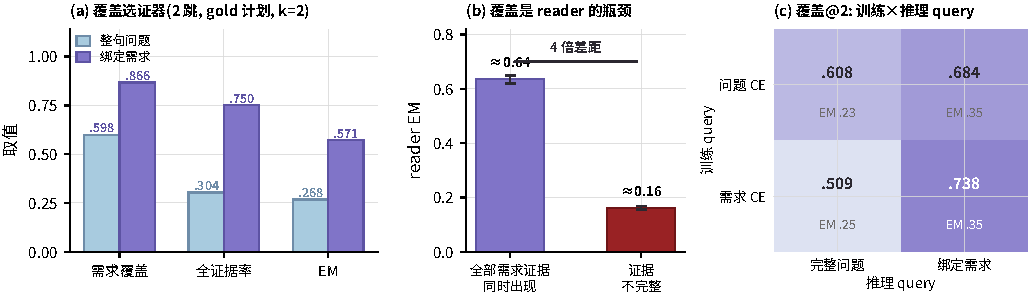
\includegraphics[width=\textwidth]{figures/fig5_coverage_bottleneck.pdf}
  \caption{覆盖而非单段相关性是端到端瓶颈。(a) gold 计划、$k{=}2$ 的 2 跳子集上,
  绑定查询槽的覆盖选证器将需求覆盖率 $0.598\!\to\!0.866$、全证据率 $0.304\!\to\!0.750$、
  EM $0.268\!\to\!0.571$;(b) 按证据完整度分层,全部需求证据同时出现时 reader EM 约
  $0.62$--$0.65$,证据不完整时仅约 $0.155$--$0.169$(误差条为报告区间);
  (c) 需求 CE 与问题 CE 使用相同训练题与正负例、仅改变训练/推理 query:
  推理侧换成绑定需求的覆盖收益远大于训练侧(如 $0.509\!\to\!0.738$ 对 $0.684\!\to\!0.738$)。}
  \label{fig:coverage}
\end{figure*}

% ---------- Figure 6 端到端比较(双栏) ----------
\begin{figure*}[t]
  \centering
  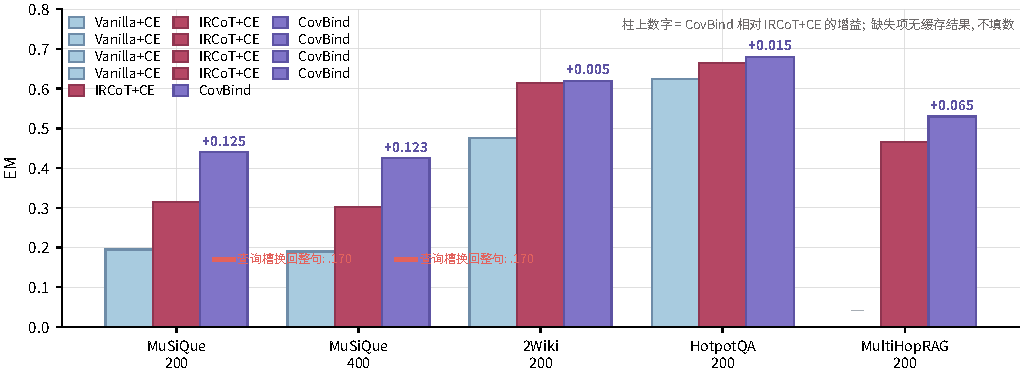
\includegraphics[width=\textwidth]{figures/fig6_end_to_end.pdf}
  \caption{跨数据集端到端比较(EM)。柱上数字为 CovBind 相对 IRCoT+CE 的增益:
  MuSiQue 上稳定显著($+0.125$/$+0.123$),2Wiki 与 HotpotQA 基本持平
  ($+0.005$/$+0.015$),MultiHopRAG 为边缘收益($+0.065$)。
  深红色横线为将 CovBind 查询槽换回整句问题的反事实(MuSiQue:$0.170$);
  MultiHopRAG 的 Vanilla+CE 无缓存结果,以“---”标示,不填入数字。}
  \label{fig:e2e}
\end{figure*}

% ---------- Figure 7 适用性判据(单栏) ----------
\begin{figure}[t]
  \centering
  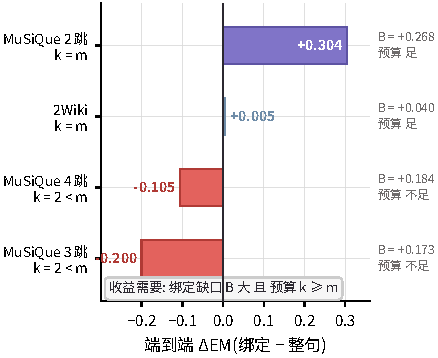
\includegraphics[width=\columnwidth]{figures/fig7_applicability.pdf}
  \caption{适用性判据:绑定收益需要“绑定缺口 $B$ 大”且“预算 $k\ge m$”同时满足。
  MuSiQue 2 跳($B{=}{+}0.268$,$k{=}m$)获得 $+0.304$ EM;2Wiki 缺口小,
  收益接近零;而 MuSiQue 3/4 跳在 $k{=}2<m$ 时,逐需求取证挤占末跳预算,
  端到端 EM 反而下降 $-0.200$/$-0.105$。}
  \label{fig:applicability}
\end{figure}

% ---------- Figure 8 多方法端到端比较(双栏) ----------
\begin{figure*}[t]
  \centering
  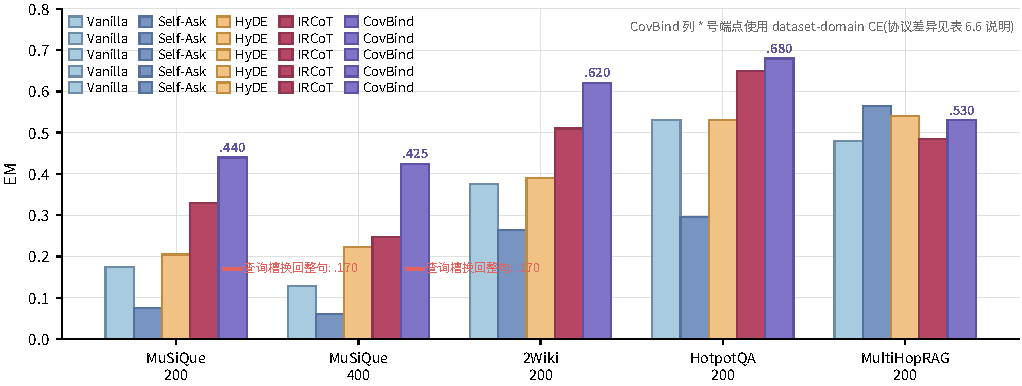
\includegraphics[width=\textwidth]{figures/fig8_method_comparison_full.pdf}
  \caption{多方法端到端比较（EM，对应正文表 6.6）。Vanilla、Self-Ask、HyDE、IRCoT 与
  CovBind 逐数据集对照，深红色横线为 CovBind-whole-query 反事实（MuSiQue：$.170$）。
  CovBind 列 $*$ 号端点使用 dataset-domain CE，与 zero-shot 基线保留协议差异；
  严格因果结论以同 matcher 的 whole-query 反事实为准。}
  \label{fig:method-comp}
\end{figure*}

% ---------- Figure 9 机制复验与跨数据集可达性(双栏) ----------
\begin{figure*}[t]
  \centering
  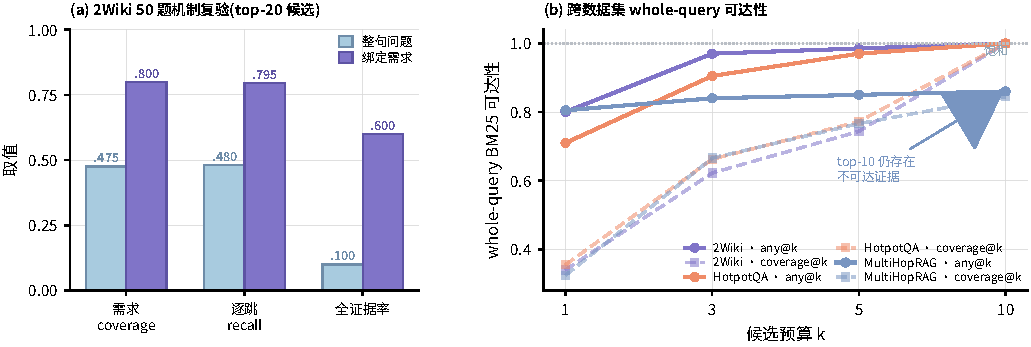
\includegraphics[width=\textwidth]{figures/fig9_mechanism_crossreach.pdf}
  \caption{(a) 2Wiki 50 题机制复验（top-20 候选、gold-binding 协议）：绑定使需求 coverage
  $.475\!\to\!.800$、逐跳 recall $.480\!\to\!.795$、全证据率 $.100\!\to\!.600$；
  (b) whole-query BM25 可达性随预算 $k$ 的变化（实线 any@k，虚线 coverage@k）：
  2Wiki 与 HotpotQA 在 $k{=}10$ 饱和至 $1.0$，MultiHopRAG 的 any@k 仍只有 $.860$，
  存在不可达证据，与方法的结构性适用条件一致。}
  \label{fig:mech-reach}
\end{figure*}

% ---------- Figure 10 绑定质量与单跳控制(单栏) ----------
\begin{figure}[t]
  \centering
  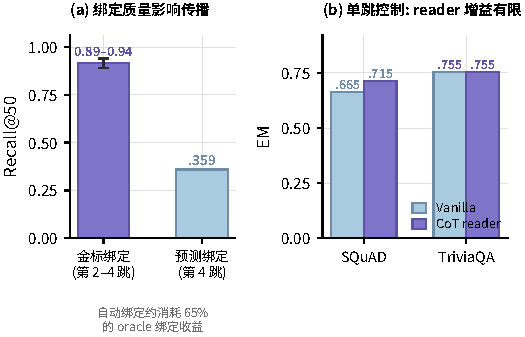
\includegraphics[width=\columnwidth]{figures/fig10_binding_quality_singlehop.pdf}
  \caption{(a) 绑定质量影响收益传播：金标绑定下后续跳 Recall@50 可达 $0.89$--$0.94$，
  预测绑定后第 4 跳可回落至 $.359$，自动绑定约消耗 65\% 的 oracle 绑定收益；
  (b) 单跳控制（SQuAD/TriviaQA，每题 10 段池）：CoT reader 增益有限
  （SQuAD $+0.050$，TriviaQA 持平），多跳收益主要由绑定查询槽带来。}
  \label{fig:binding-quality}
\end{figure}

% ---------- Figure 11 负结果(单栏) ----------
\begin{figure}[t]
  \centering
  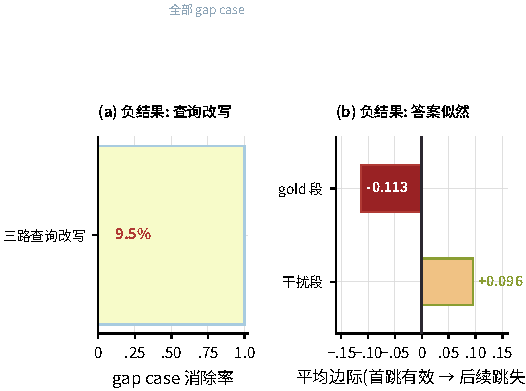
\includegraphics[width=\columnwidth]{figures/fig11_negative_results.pdf}
  \caption{负结果中的可量化项。(a) 三路查询改写在测量的 gap case 上仅消除 9.5\%；
  (b) 答案似然边际效用首跳有效、后续跳失效：gold 段平均边际为 $-0.113$，
  干扰段为 $+0.096$。LLM 绝对充分性判断低于 base CE、绑定门控/共识/回滚等
  未形成稳定收益，因无可比数字不以图呈现。}
  \label{fig:negative}
\end{figure}
